\section{回路設計}
今回設計した駆動部,距離センサ部,マイコン周辺部の回路図を\refig{dc_motor_unit},\refig{sensor_unit},\refig{control_unit}にそれぞれ示す.
また回路制作に使用した主要な部品の一覧を\reftab{circuit_parts}に示す.
さらに駆動系の回路に関してその詳細な仕様や構成について以下で述べる.

\begin{figure}[h]
\centering
\includegraphics[scale=0.4]{picture/eps/dc_motor_unit.eps}
\caption{駆動部}
\label{fig::dc_motor_unit}
\end{figure}

\begin{figure}[b]
\centering
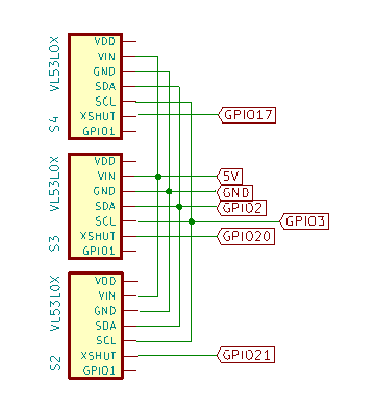
\includegraphics[scale=1]{picture/eps/sensor_unit.eps}
\caption{距離センサ部}
\label{fig::sensor_unit}
\end{figure}

\begin{figure}[h]
\centering
\includegraphics[scale=0.5]{picture/eps/control_unit.eps}
\caption{マイコン周辺部}
\label{fig::control_unit}
\end{figure}

\clearpage

\begin{table}
    \caption{電気回路用部品}
    \label{tab::circuit_parts}
    \begin{center}
    \footnotesize
   \begin{tabular}{ | l | l | c || l |}\hline
タイプ               &部品名                                         &数&用途   \\ \hline\hline
マイコン          &Raspberry Pi3 Model B                            &1&制御用           \\ \hline
DCモータ          &RP380                                   &1&後輪モータ駆動用   \\    \hline
モータドライバ      &MD10C R3                                        &1&後輪モータ制御用   \\ \hline
距離センサ         &VL53L0X Time-of-Flight                           &3&距離計測用   \\ \hline
フォトリフレクタ     &QTR-1RC フォトリフレクタ・モジュール              &3&ゴールライン計測用   \\ \hline
DC-DCコンバータ     &BTD05-05S200D                                     &1&降圧用   \\ \hline
コンデンサ          &セラミックコンデンサ$1000\unit{pF}50\unit{V}$ &1&後輪モータのノイズ除去用   \\ \cline{2-4}
                  &OSコンデンサ $10\unit{V}47\unit{\mu F}$                          &2&DC-DCコンバータのノイズ除去用    \\ \hline
ロータリーエンコーダ &RE30E-500-213-1                                   &1&ロボカーの速度計測用   \\ \hline
バッテリ          &Powers Max 4000 Ni-MH $7.2\unit{V}$                        &1&DCモータ,サーボモータ用の電源\\ \cline{2-4}
                  &$4000\unit{mAh}$ 6CELL ニッケル水素バッテリ                &1&Raspberry Pi3 ModelB用の電源    \\ \hline
サーボモータ        &GWS03T/2BBMG                                &1&ステアリング用   \\    \hline

	   \end{tabular}
	\end{center}
\end{table}





\subsection{全体の回路構成}

今回設計した回路では$7.2\unit{V}$バッテリと$5\unit{V}$バッテリの2つを用いており,$7.2\unit{V}$バッテリはまず分流を行い一方をDC-DCコンバータを用いて$7.2\unit{V}$から$5\unit{V}$に降圧してサーボモータに供給し,もう一方をDCモータドライバに供給している.$5\unit{V}$バッテリはRaspberryPi3 Model Bにのみ電源を供給している.このような回路構成をとることで,RaspberryPi3 Model Bへの電源供給に対してフィルタを用いたノイズ対策を行う必要がなく安定した動作を行うことができるというメリットがある\cite{motor}.


\subsection{駆動部の回路}
\refig{dc_motor_unit}は車体駆動部回路を示している.駆動部回路は後輪駆動部回路とステアリング回路から構成されている.以下で詳細について説明する.


\subsubsection{後輪駆動部の回路}
後輪駆動部の回路は主にモータドライバとDCモータから構成されている.以下にその仕様を示す.DCモータには,ノイズを軽減するためにセラミックコンデンサを取り付けた\cite{motor}.
\begin{description}
    \item[モータドライバ\textless MD10CR3(Cytron technologies社製)\textgreater \cite{motordriver}]\mbox{}\\
    \vspace{-5mm}
        \begin{itemize}
            \item 対応モータ電圧: DC $5\unit{V}-25\unit{V}$
            \item 最大電流  : $13\unit{A}$
            \item ロジック入力電圧: $3.3\unit{V}-5\unit{V}$
        \end{itemize}
     \item[DCモータ\textless RP380(マブチモーター社製)\textgreater\cite{R380}]\mbox{}\\
     \vspace{-5mm}
         \begin{itemize}
            \item 適正電圧:$7.2\unit{V}$
            \item 適正電圧・負荷時の消費電流: $2.9\unit{A}$
        \end{itemize}
\end{description}

\newpage

\subsubsection{ステアリング回路}
ステアリング用の回路ではサーボモータと降圧を行うためのDC-DCコンバータから構成されている.以下にその仕様を示す.ここで,サーボモータのGNDはRaspberryPi3 ModelBのそれと共通である.DC-DCコンバータは内部でディジタルスイッチングを行っているため,ノイズが生じてしまう\cite{dcdc}.本回路ではこのようなノイズ成分を平滑化するために電解コンデンサ(OSコンデンサ$10\unit{V}47\unit{\mu F}$)を用いた\refig{dcdc_unit}の回路を作成した\cite{dcdcconverter}.

\begin{description}
    \item[DC-DCコンバータ(Bellnix社製)\textless BTD05-05S200D\textgreater \cite{dcdcconverter}]\mbox{}\\
    \vspace{-5mm}
        \begin{itemize}
            \item 入力電圧: DC $4.5\unit{V}-9\unit{V}$
            \item 出力電圧: $0\unit{mA}-2000\unit{mA}$
            \item 出力電流: $3.3\unit{V}-5\unit{V}$
            \item 効率: 84 \%
        \end{itemize}
     \item[サーボモータ\textless GWS03T/2BBMG\textgreater]\mbox{}\\
    \vspace{-5mm}
         \begin{itemize}
            \item 駆動電圧: DC $4.8\unit{V}-6\unit{V}$
        \end{itemize}
\end{description}


\begin{figure}[h]
\centering
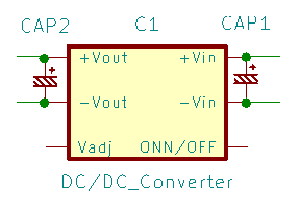
\includegraphics[scale=0.8]{picture/eps/dcdc_unit.eps}
\caption{DC-DCコンバータの回路図}
\label{fig::dcdc_unit}
\end{figure}
